\documentclass[12pt]{article}
% Full article preamble (duplicated, no common file)
\usepackage{fontspec}
\usepackage[a4paper,margin=2.5cm,includefoot]{geometry}
\usepackage{polyglossia}
\usepackage{amsmath}
\usepackage{amssymb}
\usepackage{xcolor}
\usepackage{fancyhdr}
\usepackage{graphicx}
\usepackage{listings}
\usepackage[most]{tcolorbox}
\usepackage{pifont}
\usepackage{enumitem}
\usepackage{titlesec}
\usepackage[bottom]{footmisc}
\usepackage{titling}
\usepackage{minted}
\usepackage{etoolbox}
\usepackage{array}
\usepackage{extsizes}

\newfontfamily\emoji{Segoe UI Emoji}

\pagestyle{fancy}

\setmainlanguage[numerals=western]{arabic}
\setotherlanguage{english}
\newfontfamily\arabicfont[Script=Arabic]{Amiri}
\newfontfamily\arabicfonttt[Script=Arabic]{Courier New}

\lstset{
  language=[Sharp]C,
  numbers=left,
  stepnumber=1,
  numbersep=8pt,
  frame=single,
  basicstyle=\ttfamily\small,
  keywordstyle=\color{blue},
  stringstyle=\color{red},
  commentstyle=\color{green!50!black}
}

\newif\ifdetailed
\ifdefined\setdetailed
  \setdetailed
\fi

\newif\ifwithsols
\ifdefined\setwithsols
  \setwithsols
\fi

% unified tcolorboxes for articles
\tcbset{colback=white, colframe=black, fonttitle=\bfseries, boxrule=0.8pt}
\newtcolorbox{boxDef}[1][]{colback=blue!5!white,colframe=blue!75!black,
  title={{\emoji📘} تعريف\ifx\\#1\\\else ~#1\fi :}}
\newtcolorbox{boxExercise}[1][]{colback=cyan!5!white,colframe=cyan!70!black,
  title={{\emoji🧩} تمرين\ifx\\#1\\\else ~#1\fi :}}
\newtcolorbox{boxExample}[1][]{colback=yellow!5!white,colframe=orange!90!black,
  title={{\emoji📝} مثال\ifx\\#1\\\else ~#1\fi :}}
\newtcolorbox{boxNote}[1][]{colback=gray!10!white,colframe=black,
  title={{\emoji✨} ملاحظة\ifx\\#1\\\else ~#1\fi :}}
\newtcolorbox{boxAttention}[1][]{colback=magenta!10!white,colframe=magenta!80!black,
  title={{\emoji🔔} تنبيه\ifx\\#1\\\else ~#1\fi :}}
\newtcolorbox{boxWarning}[1][]{colback=red!5!white,colframe=red!75!black,
  title={{\emoji⚡} ملاحظة هامة\ifx\\#1\\\else ~#1\fi :}}
\newtcolorbox{boxSolution}[1][]{colback=green!5!white,colframe=green!60!black,
  title={{\emoji✅} حل\ifx\\#1\\\else ~#1\fi :}}
\newtcolorbox{boxSymbol}[1][]{colback=purple!5!white,colframe=purple!70!black,
  title={{\emoji🔣} رمز\ifx\\#1\\\else ~#1\fi :}}

\tcbset{simplecode/.style={ colback=gray!5, colframe=black!50, boxrule=0.4pt, arc=2pt, left=4pt,right=4pt,top=4pt,bottom=4pt}}
\newenvironment{boxCode}{\begin{tcolorbox}[simplecode]}{\end{tcolorbox}}

\newcolumntype{C}[1]{>{\centering\arraybackslash}p{#1}}

% redefine spaces after titles
\makeatletter
\renewcommand{\@maketitle}{%
  \begin{center}
    {\huge \bfseries \@title \par}%
    \vskip 0.2em % space between title and author
    {\large \@author \par}%
    % \vskip 0.2em % space between author and date
    % {\normalsize \@date \par}%
  \end{center}
}
\makeatother

\fancyhf{} % clear default
\fancypagestyle{plain}{
  \fancyhf{}
  \fancyhead[L]{مدرسة التسامح الشاملة}
  % \fancyhead[L]{
\includegraphics[height=1cm]{../../../images/logoTasamoh.png}}
  \fancyhead[R]{الأستاذ محمود اغبارية}
  \fancyfoot[C]{\thepage}
}

\fancyhead[L]{مدرسة التسامح الشاملة}
\fancyhead[R]{الأستاذ محمود اغبارية}
\fancyfoot[C]{\thepage}
% \date{\today}

\setcounter{tocdepth}{3} % only section subsection and subsubsection in TOC


% ----------------------


% \begin{document}

% \maketitle

% % \clearpage  % start TOC on a new page
% % \renewcommand{\contentsname}{جدول المحتويات}
% % \tableofcontents
% % \clearpage

% \part*{part 1} % the * prevents numbering
% \section*{مقدمة}
% \subsection*{مثال رياضي}
% \subsubsection*{مثال فرعي}
% \paragraph*{ paragraph 1}
% \subparagraph*{sub paragraph 1}

% \ifdetailed
% \begin{english}
% \begin{minted}{csharp}
% // C# Example
% \end{minted}
% \end{english}
% \fi

% OLD WAY
% \ifdetailed
% \begin{english}
% \begin{lstlisting}
% // C# Example
% \end{lstlisting}
% \end{english}
% \fi

% % 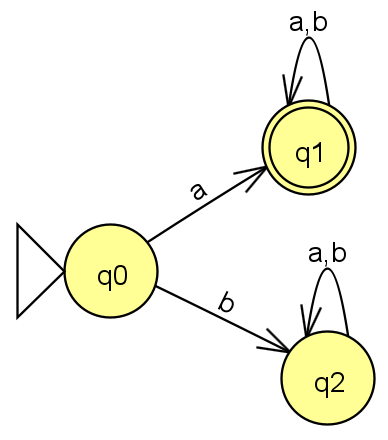
\includegraphics[width=0.2\textwidth]{../../../images/DFAs/ex1_q1.png}



% \vspace{3cm}
% \begin{flushleft}
% أرجو لكم وقتًا ممتعًا.

% الأستاذ محمود اغبارية.
% \end{flushleft}


% \end{document}


\begin{document}

\title{درس مفصَّل حول جملة \emph{\textenglish{if}} في لغة C\#}
\author{مستند تعليمي مُعد بناءً على عدة عروض تقديمية}
\date{}

\maketitle
\thispagestyle{fancy}

\section*{مقدمة}

تُعدُّ الجملة الشرطية \textenglish{if} من أهم البنى في لغات البرمجة، إذ تسمح للبرنامج باتخاذ قرارات وتنفيذ مقاطع من التعليمات فقط عندما يتحقق شرط معيّن. يمكن النظر إلى الشرط على أنه ``جملة منطقية'' أو ``تعبير بولياني''؛ أي عبارة قيمتها إما \emph{صحيح} أو \emph{خطأ}. بحسب العروض التعليمية التي اطلعنا عليها، يُعرَّف التعبير البولياني بأنه عبارة ``يمكن إسناد القيمة \emph{صح} أو \emph{خطأ} لها، ولا يمكن أن تأخذ القيمتين معاً''. ومن الأمثلة على جمل منطقية: ``إسرائيل تقع في الشرق الأوسط'' أو المقارنة الرياضية \verb|5 > 7|. بينما عبارة مثل ``ما أخبارك؟'' لا يمكن وصفها بأنها جملة منطقية؛ لأنها لا تحمل قيمة \emph{صح} أو \emph{خطأ}.

\section{بناء جملة \textenglish{if} في C\#}

\subsection{تنفيذ مشروط}

عند الحاجة إلى تنفيذ مجموعة أوامر بناءً على تحقق شرط معين، نستخدم جملة \textenglish{if}. ذكرت العروض أن ``\emph{التنفيذ المشروط} هو حالة نرغب فيها بتنفيذ أو تخطي مجموعة تعليمات في البرنامج، وتكون القرارات مبنية على تحقق شروط معيّنة''. يمكن أن تكون الجملة على الشكل الآتي:

\begin{english}
\begin{minted}{csharp}
if (condition)
{
    // Executed when the condition is true
}
\end{minted}
\end{english}

إذا تحقق \verb|condition| (أي كانت قيمته \texttt{true}) تُنفَّذ التعليمات الموجودة بين الأقواس $\{\}$، وإلا تُتجاهل تلك التعليمات ويستمر البرنامج بالعمل.

\subsection{اختيار بين فرعين (\textenglish{if-else})}

في بعض الأحيان نحتاج إلى تنفيذ أحد فرعين من الأوامر فقط. في هذه الحالة نستعمل \textenglish{if-else}. ذكرت العروض أن ``برمجة القرار هي حالة يختار فيها البرنامج تنفيذ مقطع \emph{أ} أو مقطع \emph{ب} لكن ليس كلاهما''. الصيغة العامة:

\begin{english}
\begin{minted}{csharp}
if (condition)
{
    // Statements when the condition is true
}
else
{
    // Statements when the condition is false
}
\end{minted}
\end{english}

مثال بسيط: إذا أردنا طباعة "1" عندما يكون المتغيّر \texttt{x} أكبر من \texttt{0}، وإلا نطبع "سالب أو صفر":

\begin{english}
\begin{minted}{csharp}
Console.Write("Enter a number: ");
int x = int.Parse(Console.ReadLine());
if (x > 0)
{
    Console.WriteLine("Positive");
}
else
{
    Console.WriteLine("Negative or zero");
}
\end{minted}
\end{english}

\subsection{الكتلة $\{\}$ والوضوح}

عندما يتطلب الشرط تنفيذ أكثر من تعليمة واحدة، نحيط تلك التعليمات بكتلة تبدأ بقوس $\{$ وتنتهي بقوس $\}$. أكدت العروض أن ``الكتلة هي عبارة عن مجموعة من التعليمات تُعامل كتعليمة واحدة، وتبدأ بـ$\{$ وتنتهي بـ$\}$''. لا يوجد حد لعدد التعليمات داخل الكتلة، وإذا كانت الكتلة تأتي مباشرة بعد \textenglish{if} فيُعامل البرنامج الكتلة كتعليمة واحدة.

لتحسين القراءة، يفضّل استعمال مسافة بادئة (\emph{indentation}) بحيث توضع جملة \textenglish{else} مباشرة تحت \textenglish{if} الخاصة بها، وتكون التعليمات داخل الكتلة مزاحة إلى اليمين بمقدار \texttt{Tab}. بعض المترجمات تتيح وضع القوس المفتوح $\{$ في نهاية سطر \textenglish{if} أو في السطر التالي؛ لكن يوصى بوضعه في السطر التالي لتجنّب نسيان إغلاق الكتلة.

\section{التعابير المنطقية والمُعاملات}

التعابير المنطقية يمكن أن تكون بسيطة (مثل \verb|x > y|) أو مركبة. في الحالة المركبة نستخدم المعاملات المنطقية \emph{و} (\texttt{\&\&}) و\emph{أو} (\texttt{||}) و\emph{ليس} (\texttt{!}). العروض تُعرِّف هذه المعاملات بوضوح: ``المعاملات المنطقية هي: \emph{و} (\textenglish{and}، يُمثَّل بـ\texttt{\&\&})، \emph{أو} (\textenglish{or}، يُمثَّل بـ\texttt{||})، و\emph{ليس} (\textenglish{not}، يُمثَّل بـ\texttt{!})''.

مثال على تعبير منطقي مركَّب في C\#:

\begin{english}
\begin{minted}{csharp}
bool result = (x < y) && (x + y < z) || (x < 0);
\end{minted}
\end{english}

لحساب نتيجة هذا التعبير، نستبدل المتغيرات بقيمها ثم نحسب القيم المنطقية. في العرض تم شرح ذلك خطوة بخطوة: إذا كان \verb|x = -4| و\verb|y = 6| و\verb|z = 3| فإن التعويض يعطي \verb|-4 < 6 && -4 + 6 < 3 || -4 < 0|، والذي يقيَّم إلى \verb|True&&True||True| ثم إلى \verb|True|.

\subsection{أولوية التقييم}

عند وجود أكثر من معامل منطقي في تعبير واحد، يكون لمعامل \emph{ليس} \verb|!| الأولوية الأعلى، ثم \emph{و} \verb|&&|، ثم \emph{أو} \verb|||. يمكن استخدام الأقواس \verb|()| لتحديد ترتيب الحساب بشكل واضح. من الجيد أن تُستَخدم الأقواس عند كتابة تعبيرات معقَّدة لتحسين القراءة ولتفادي الأخطاء.

\subsection{المتغيرات البوليانية}

يسمح C\# بتعريف متغيرات من نوع \texttt{bool} تأخذ القيمتين \texttt{true} أو \texttt{false} فقط. يعرَّف المتغير البولياني بأنه ``متغيّر يمكنه أخذ قيمة \emph{صحيح} أو \emph{خطأ} فقط''. يمكن إسناد قيمة مباشرة أو نتيجة تعبير منطقي إلى متغير من هذا النوع:


\begin{english}
\begin{minted}{csharp}
bool big = num1 > num2;
bool equals = num1 == num2;
\end{minted}
\end{english}

هذا يجعل الكود أكثر وضوحاً، ويمكن استخدام هذه المتغيرات في الشروط مباشرة.

\section{التداخل (\textenglish{Nested if}) والمشكلة الكلاسيكية لـ\textenglish{else} المفقودة}

من الممكن كتابة جملة \textenglish{if} داخل جملة \textenglish{if} أخرى. يشار إلى ذلك في العروض باسم ``تداخل الجمل الشرطية'' ويُذكر أن ``التعليمة التي تُنفذ بعد \textenglish{if} أو بعد \textenglish{else} يمكن أن تكون أي تعليمة في اللغة، بما في ذلك جملة \textenglish{if} أخرى''. يمكن أن يكون التداخل في الفرع الأول (بعد \textenglish{if}) أو في الفرع الثاني (بعد \textenglish{else}).

مثال على تداخل لاختيار أصغر ثلاثة أعداد مختلفة هو الخوارزمية التالية (مستقاة من العروض):


\begin{english}
\begin{minted}{csharp}
int a, b, c;
// Assume a, b, c were read from the user
int smallest;
if (a < b)
{
    if (a < c)
        smallest = a;
    else
        smallest = c;
}
else
{
    if (b < c)
        smallest = b;
    else
        smallest = c;
}
Console.WriteLine($"Smallest is {smallest}");
\end{minted}
\end{english}

\paragraph{مشكلة \textenglish{else} المفقودة} عند كتابة جمل \textenglish{if} متداخلة، قد يحدث التباس حول أي \textenglish{else} يتبع أي \textenglish{if}. يُسمى هذا ``مشكلة \textenglish{else} المفقودة'' أو \textenglish{dangling else}. في إحدى الشرائح أُعطي المثال التالي:

\begin{english}
\begin{minted}{csharp}
if (num > 0)
    if (num < 150)
        num = Math.Sqrt(num);
    else;
else
    num = 0;
\end{minted}
\end{english}

هنا يبدو أن عبارة \textenglish{else} الأولى مرتبطة بـ\textenglish{if (num < 150)}، مما يؤدي إلى سلوك غير مقصود. ولحل المشكلة يجب استخدام الأقواس لتوضيح التراكيب:

\begin{english}
\begin{minted}{csharp}
if (num > 0)
{
    if (num < 150)
        num = Math.Sqrt(num);
}
else
{
    num = 0;
}
\end{minted}
\end{english}

هذا المثال مأخوذ من العروض التي تناقش ``مشكلة \textenglish{ELSE} المفقودة''.

\section{أمثلة وبرامج تطبيقية}

فيما يلي بعض الأمثلة العملية المقتبسة من العروض والتي تساعد على فهم كيفية استخدام \textenglish{if} في C\#.

\subsection{حساب مساحة حلقة بين دائرتين}

المطلوب كتابة برنامج يقرأ نصف قُطر دائرتين ذواتي مركز واحد ويحسب مساحة الحلقة الواقعة بينهما. إذا كان نصف القطر الأول أكبر من الثاني نحسب \(\pi r_{1}^{2} - \pi r_{2}^{2}\)، والعكس صحيح. الفكرة أن نستخدم \textenglish{if} لاختيار أي مساحة نطرح من الأخرى.

\begin{english}
\begin{minted}{csharp}
Console.Write("Enter first radius: ");
double r1 = double.Parse(Console.ReadLine());
Console.Write("Enter second radius: ");
double r2 = double.Parse(Console.ReadLine());
double ringArea;
if (r1 > r2)
{
    ringArea = Math.PI * r1 * r1 - Math.PI * r2 * r2;
}
else
{
    ringArea = Math.PI * r2 * r2 - Math.PI * r1 * r1;
}
Console.WriteLine($"Ring area = {ringArea}");
\end{minted}
\end{english}

\subsection{تصنيف الأعداد}

\paragraph{مثال 1: العدد أكبر من مئة؟} اكتب برنامجاً يقرأ عدداً صحيحاً ويطبع ``كبير'' إذا كان العدد أكبر من 100. يمكن تمديد البرنامج ليطبع ``صغير'' إذا كان أقل من 100، ثم نضيف حالة مساواة لتغطية جميع الاحتمالات.

\begin{english}
\begin{minted}{csharp}
int n = int.Parse(Console.ReadLine());
if (n > 100)
    Console.WriteLine("Large");
else if (n < 100)
    Console.WriteLine("Small");
else
    Console.WriteLine("Equals 100");
\end{minted}
\end{english}

\paragraph{مثال 2: موجب، سالب أم صفر؟} لقراءة عدد ما وتحديد ما إذا كان موجباً أو سالباً أو صفراً نستعمل سلسلة \textenglish{if‑else if‑else} كما يلي:

\begin{english}
\begin{minted}{csharp}
double x = double.Parse(Console.ReadLine());
if (x > 0)
    Console.WriteLine("Positive");
else if (x < 0)
    Console.WriteLine("Negative");
else
    Console.WriteLine("Zero");
\end{minted}
\end{english}

\paragraph{مثال 3: مقارنة عددين} لقراءة عددين وطباعة ``متساويان'' إذا كانا متساويين و``مختلفان'' otherwise، يمكن استخدام عامل المساواة \verb|==|:


\begin{english}
\begin{minted}{csharp}
Console.Write("Enter first number: ");
int a = int.Parse(Console.ReadLine());
Console.Write("Enter second number: ");
int b = int.Parse(Console.ReadLine());
if (a == b)
    Console.WriteLine("Equal");
else
    Console.WriteLine("Different");
\end{minted}
\end{english}

\subsection{ترتيب ثلاثة أعداد}

يُعتبر ترتيب ثلاثة أعداد من الأصغر إلى الأكبر مثالاً ممتازاً على التداخل. يمكن استخدام الطريقة المباشرة كما في المثال السابق لاختيار الأصغر، ثم يمكن مقارنة العددين المتبقيين. العروض تذكر مخططاً يتيح مقارنة كل زوج من الأعداد واستخلاص النتيجة. برنامج مبسَّط لفرز ثلاثة أعداد هو:


\begin{english}
\begin{minted}{csharp}
int a = int.Parse(Console.ReadLine());
int b = int.Parse(Console.ReadLine());
int c = int.Parse(Console.ReadLine());
// Ensure that 'a' holds the smallest value
if (a > b)
{
    int temp = a; a = b; b = temp;
}
if (a > c)
{
    int temp = a; a = c; c = temp;
}
// Now 'a' is the smallest; order b and c
if (b > c)
{
    int temp = b; b = c; c = temp;
}
Console.WriteLine($"Sorted ascending: {a}, {b}, {c}");
\end{minted}
\end{english}

\section{تمارين مقترحة}

بالإضافة إلى الأمثلة السابقة، تقترح العروض التعليمية مجموعة من التمارين لتثبيت فهم الجملة الشرطية. فيما يلي بعض التمارين المقترحة:

\begin{enumerate}
  \item كتابة برنامج يقرأ ثلاثة أعداد صحيحة ويطبع العدد الأصغر من بينها.
  \item كتابة برنامج يقرأ ثلاثة أعداد صحيحة مختلفة ويعرضها مرتبة من الأصغر إلى الأكبر.
  \item كتابة برنامج يقرأ عددًا صحيحًا \(n\)؛ إذا كان \(n\) أكبر من \(7\) يطبع ``كثير''، وإذا كان أقل من \(7\) يطبع ``قليل''، وإذا كان مساويًا لـ\(7\) يطبع ``تماماً''.
  \item كتابة برنامج يتحقق من صحة رقم ثلاثي الأرقام: اطبع رسالة خطأ إذا كان أصغر من \(100\) أو أكبر من \(999\). هذا التمرين يتطلّب استخدام معامل \textenglish{or} \texttt{||} في الشرط، كما ظهر في العروض.
  \item كتابة برنامج يحسب نوع مثلث بناءً على أطوال أضلاعه: إذا كانت إحدى الضلعين سلبية أو صفرًا تُطبع رسالة خطأ (``الضلع يجب أن يكون عدداً موجباً''). وإلا تُستخدم الشروط لتحديد ما إذا كان متساوي الأضلاع أو متساوي الساقين أو مختلف الأضلاع.
  \item استخدام متغيّر بولياني \verb|valid| لتحديد ما إذا كان إدخال المستخدم صحيحاً. ثم استخدام \verb|if (valid)| أو \verb|if (!valid)| لاتخاذ القرار المناسب.
\end{enumerate}

\section*{خاتمة}

يُعد فهم جملة \textenglish{if} في لغة C\# أمراً أساسياً لكل مبرمج. تبدأ هذه الجملة بالتعبير عن شرط منطقي يُحدِّد ما إذا كان مقطع معين من الكود سينفّذ أم لا، ويمكن توسيعها باستخدام \textenglish{else} و\textenglish{else if} لتغطية جميع الاحتمالات. أوضحت العروض ضرورة استخدام الأقواس لتجنّب الغموض في التراكيب المتداخلة، وأهمية ترتيب الشفرة واستخدام المسافات البادئة لتحسين القراءة. كما عرَّفت المعاملات المنطقية والمتغيرات البوليانية، وقدمت أمثلة وتمارين عملية تساعد على ترسيخ المفاهيم. من خلال الممارسة والتمرين ستصبح القدرة على كتابة شروط دقيقة وواضحة جزءاً طبيعياً من مهاراتك البرمجية.

\end{document}
